\documentclass[12pt]{article}
\usepackage[utf8]{inputenc}
\usepackage{listings}
\usepackage{hyperref}
\usepackage{graphicx}


\lstdefinestyle{output}{
    breaklines=true,
    showspaces=false,
    basicstyle=\footnotesize,
    breakatwhitespace=false
}


\begin{document}

\lstset{style=output}
\setlength\parindent{0pt}

% title page
\begin{titlepage}
    \begin{center}
        \vspace*{1cm}

        \Huge
        \textbf{Predicting Pathogenicity using Aberrant Splicing Predictions of Single Nucleotide Variants in Autism Spectrum Disorder}\\


        \vspace{0.5cm}
        \Large
        \textbf{Bioinformatics Laboratory, BIMM 185}

        \vspace{1.5cm}
        \textbf{Kevin Chau}

        \vfill

        \Large
        University of California, San Diego\\
        16 June 2017
    \end{center}
\end{titlepage}

\thispagestyle{plain}
\begin{center}
    \textbf{Abstract}
\end{center}
Distributions of splicing likelihood scores for single nucleotide variants 
(SNVs) were analyzed with the hopes that these scores could be used to 
predict their pathogenicity, defined as a pathogenicity score multiplied by a 
risk score for that gene. SNVs implicated in autism as well as those found in
control phenotypes were gathered and scored for their likelihood to cause 
cassette exon skipping and their pathogenicity. Gene coexpression networks
were constructed for affected genes per eight developmental periods using
publicly available RNA-seq data. Genes were scored for risk, per period, 
based on relative numbers of coexpression partners. Figures show that there is
no difference in the distribution of splicing scores between SNVs implicated
in autism versus control, nor was there any correlation between the splice
score and pathogenicity (modified by the gene risk score).

\pagebreak

% begin report contents
\section{Introduction}
Prediction of pathogenicity of genetic variants is paramount to current 
understanding of diseases with heavy genetic influence and, by extension,
development of treatments. In addition, it has been shown that aberrant 
splicing can have major contributions to expression of disease phenotypes, 
likely due to a propensity to disrupt biological pathways through alteration 
of gene products. Therefore, one might deduce that variants 
predicted to cause alternative splicing in genes central to biological 
processes are likely to result in the expression of the pathogenic phenotype. 
With numerous tools currently available to the public for academic use, a 
predictive model may be constructed with the hopes that the likelihood that a 
genetic variant causes aberrant splicing can be used to predict the contribution 
of that variant to development of a given disease. This knowledge could provide 
new insight into therepeutic targets at the gene or even isoform level.

\section{Data and Processing}
A list of variants classified by expressed phenotype was downloaded from 
DenovoDB, a database of nucleotide variants. Only variants tagged with the
autism phenotype and control phenotype were downloaded. Overall, the 
taken from DenovoDB included the phenotype, the nucleotide variant, chromosome,
affected gene, and starting position of the variant. This table was uploaded
to a locally hosted MySQL database for simplified querying. Since only SNVs 
were analyzed, the dataset was filtered for only mutations that substitute
one nucleotide for another. The SPIDEX splicing scoring tool was downloaded 
in order to score the nucleotide variants for their likelihood to cause 
cassette exon skipping.

\subsection{Splicing Scores with SPIDEX}
The SPIDEX tool was used to score each SNV for the likelihood that
it causes cassette exon skipping. The scoring metric used was delta PSI (dpsi),
the change in percent inclusion rate; negative values correspond to decreased
inclusion (exon skipping) and positive values correspond to increased inclusion 
(exon retention). The criteria for scoring was that the SNV must have occurred
within 300 nucleotides from a splice junction; that is, within 300 
nucleotides from an exon-to-intron or intron-to-exon transition position. Since
not all variants fell within that distance, only scorable variants were 
retained for further analysis.
\\[\baselineskip]
The SPIDEX tool is downloaded as a tab-indexed gzip-compressed file. The contents of the
file was queried using the $tabix$ utility provided by the htslib C library 
(formerly packaged with samtools). Example query and output follows:

\lstinputlisting{imports/example_spidex.txt}

with fields as Chromosome, Position, Reference Allele, Mutant Allele, dPSI, 
and Gene. 

\subsection{Pathogenicity Scores with UMD Predictor}
Pathogenicity of the given variants were scored with the web tool UMD 
Predictor. This online tool takes in a list of formatted variants and positions
and returns a score for pathogenicity of the variant for each transcript 
affected. These scores ranged from 0 to 100, with 0 being non-pathogenic and
100 being confirmed pathogenicity. These scores were converted to percentages
in order to more closely conform with the splicing scores.

\subsection{Gene Networks and Risk Analysis}
Gene coexpression networks were constructed in order to take into account
gene risk factors, with the reasoning that genes with many coexpression 
partners are more likely to play an important role in their respective 
biological pathways; disruption in their splicing would thus lead to 
pathogenicity. These coexpression networks were created using RNA-seq 
expression data from the BrainSpan database. A single network was developed for
each of eight developmental periods, since expression values are likely to
vary depending on the given stage of life. These developmental periods are as
follows: 8 weeks postconception (PCW) to 12PCW, 13PCW to 18PCW, 19PCW to 23PCW,
24PCW to 37PCW, 0 months after birth (M) to 11M, 1 year (Y) to 11Y, 12Y to 19Y,
and 21Y$^{+}$. Pairwise comparisons were performed using the Pearson 
correlation metric and all gene-gene coexpression pairs with Pearson
correlation coeffections of $\geq 0.7$ were retained. The number of 
coexpression partners for each gene was calculated and divided by the maximum
of the set, yielding the risk score for that gene. These scores were appended
to all variants that affect that gene; the relevant variant information
along with the calculated scores were all uploaded to a local MySQL database.

\section{Data Analysis}
The final dataset to analyze was compiled into a MySQL database with the 
following layout:

\lstinputlisting[language=SQL]{imports/sql_example.txt}
\pagebreak

From this data, distributions could be plotted. First, a kernel density 
estimate was performed for the frequencies of splice scores for both the 
autism phenotype and control phenotype.

\begin{figure}[ht]
\centering
    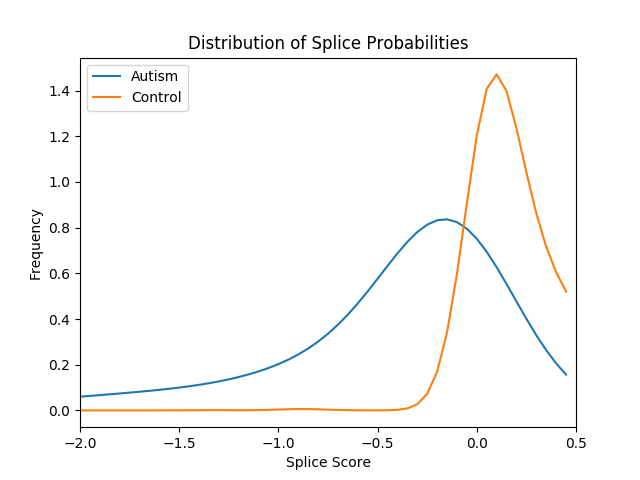
\includegraphics[width=\textwidth,height=\textheight,keepaspectratio]{../analysis/splice_distributions.png}
    \caption{Kernel density estimates of autism SNV splice scores and control SNV splice scores}
\end{figure}

\pagebreak

Scatter plots between splicing scores and pathogenicity scores
may also be drawn in order to illustrate any correlation between the two over
each developmental period and in each condition.

\begin{figure}[ht]
\centering
    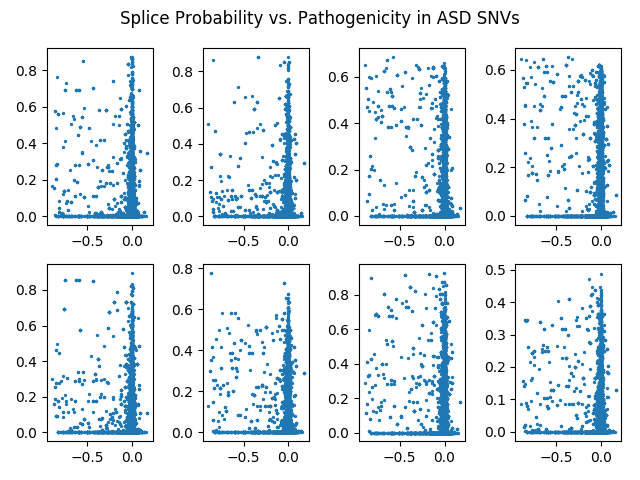
\includegraphics[width=\textwidth,height=\textheight,keepaspectratio]{../analysis/pos_corr.png}
    \caption{Splicing probabilities (x-axis) plotted against pathogenicity probabilities (y-axis) for each developmental period in SNVs implicated in autism}
\end{figure}

\begin{figure}[ht]
\centering
    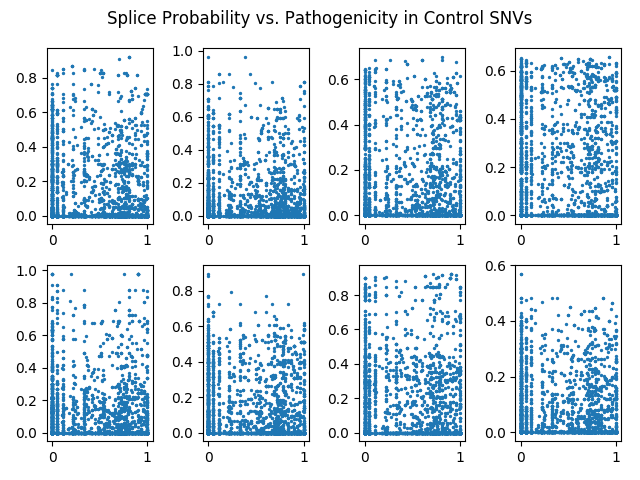
\includegraphics[width=\textwidth,height=\textheight,keepaspectratio]{../analysis/neg_corr.png}
    \caption{Splicing probabilities (x-axis) plotted against pathogenicity probabilities (y-axis) for each developmental period in control SNVs}
\end{figure}

\pagebreak

\section{Discussion}
As clearly shown by the kernel density graph, there appears to be no difference
in the distribution of autism-implicated SNVs and control SNVs; it would appear
that there is no association between splicing predictions and disease phenotype
expression. This conclusion is further supported by the splice versus 
pathogen score plots that follow. In this specific context, there is no 
correlation between splicing prediction scores and pathogenicity scores.
\\[\baselineskip]
Since there is no difference between the distributions of SNV splice 
likelihoods between the autism phenotype and control phenotypes, an inference
model incorporating these values would be completely unreliable. However,
the data and the methods used to process that data are highly specific to this 
particular context. That is, aberrant splicing of gene transcripts may 
contribute moreso to other genetic diseases besides autism spectrum disorder. 
Additionally, this analysis was performed against only single nucleotide 
variants; that is, only nucleotide substitutions were observed. Therefore,
there is likely a lower chance for actual protein modifications relative to
mutations that induce frameshifts. There was no differentiation between 
synonymous and nonsynonymous SNVs; the inclusion of synonymous SNVs could very
well skew the resulting distributions toward similarity between the phenotypes.
Furthermore, this entire process is based on the assumption that the given 
tools can reliably predict the required values. Further analysis is required
using alternative datasets and prediction tools.
\\[\baselineskip]
Although the results show that an inference model based on splice scores is not
feasible, there are still a number of tangential observations that can be made.
Interestingly, most splice scores are gathered near 0; that is, most of the 
given SNVs yield a change-in-exon-inclusion percentage of only slightly less
than 0, indicating that most of these variants do not actually induce splicing,
assuming the reliability of the SPIDEX splice predictor. With regards to the 
gene risk assessment, period four exibited the highest interconnectedness 
among its genes, which is reasonable given that this period represents the 
time interval directly before birth, giving evidence of high rates of 
neurodevelopment during this time period.

\section{Supplementary Materials}
Relevant code:\\
\href{https://github.com/kkchau/bimm185/}{https://github.com/kkchau/BIMM-185-FINAL-PROJECT/}

\end{document}
